% !TEX program = xelatex
\documentclass[a4paper,12pt, oneside]{article}
\usepackage[utf8]{inputenc}

\usepackage{graphicx} % To include images
%\usepackage{color} % To have more colors and be able to define new one
\usepackage{xcolor} % To have more colors and be able to define new one
\usepackage{afterpage} % For the page background color
\usepackage{listings} % To include code snippets
\usepackage{indentfirst} % To indent the first paragraph
\usepackage{url} % For url...
\usepackage[all]{nowidow} % To prevent widow/orphan lines
\usepackage[margin=2.5cm]{geometry} % To change the margin
\usepackage[justification=justified,singlelinecheck=false]{caption} % To left align even the single line captions
\usepackage{multicol} % Enable multi columns environment
\usepackage{subcaption} % To have two figures next to each other
\usepackage{fontspec} % For custom fonts
\usepackage{lipsum} % Lorem ipsum generator
\usepackage{layouts} %to get the text width in cm

\usepackage{tikz}
\usepackage{pgf-umlsd}
\usepgflibrary{arrows}

\setmainfont{Graublau Sans}
% \defaultfontfeatures{Scale=MatchLowercase}
% \setromanfont[Numbers=Uppercase]{FDI - GraublauSans-Regulat}
% \setmonofont[Scale=0.90,Ligatures=NoCommon]{Courier}

\definecolor{gray}{rgb}{0.4,0.4,0.4}
\definecolor{darkblue}{rgb}{0.0,0.0,0.6}
\definecolor{cyan}{rgb}{0.0,0.6,0.6}
\definecolor{rocketorange}{rgb}{1,.4,0}

\lstset{
    basicstyle=\footnotesize\ttfamily,
    breaklines=true,
    columns=fullflexible,
    showstringspaces=false,
    commentstyle=\color{gray}\upshape,
    frame=l,
    captionpos=b,
    % Line numbers
    xleftmargin={0.75cm},
    numbers=left,
    stepnumber=1,
    firstnumber=1,
    numberfirstline=true
}

\lstdefinelanguage{XML}{
  morestring=[b]",
  morestring=[s]{>}{<},
  morecomment=[s]{<?}{?>},
  stringstyle=\color{black},
  identifierstyle=\color{darkblue},
  keywordstyle=\color{cyan},
  morekeywords={xmlns,version,type,title} % list your attributes here
}

\lstdefinelanguage{JavaScript}{
  morekeywords={typeof, new, true, false, catch, function, return, null, catch, switch, var, if, in, while, do, else, case, break},
  morecomment=[s]{/*}{*/},
  morecomment=[l]//,
  morestring=[b]",
  morestring=[b]'
}

\lstdefinelanguage{HTML5}{
        language=html,
        sensitive=true,
        alsoletter={<>=-},
        otherkeywords={
        % HTML tags
        <html>, <head>, <title>, </title>, <meta, />, </head>, <body>,
        <canvas, \/canvas>, <script>, </script>, </body>, </html>, <!, html>, <style>, </style>, ><
        },
        ndkeywords={
        % General
        =,
        % HTML attributes
        charset=, id=, width=, height=,
        % CSS properties
        border:, transform:, -moz-transform:, transition-duration:, transition-property:, transition-timing-function:
        },
        morecomment=[s]{<!--}{-->},
        tag=[s]
}


% Customized commands
\newcommand{\HRule}{\rule{\linewidth}{0.5mm}}

%Acknowledgements environment
\newenvironment{acknowledgments}
  {\renewcommand{\abstractname}{Acknowledgments}
   \begin{abstract}}
  {\end{abstract}}

\begin{document}
\pagenumbering{roman}

% !TEX root = main.tex
\pagecolor{rocketorange}
\color{white}

\begin{titlepage}

\begin{center}

% Upper part of the page
\begin{minipage}{6in}
  \centering
  $\vcenter{\hbox{\includegraphics[width=55mm]{logos/logo_EPFL_White.pdf}}}$
  \hspace*{2cm}
  $\vcenter{\hbox{
\includegraphics[width=55mm]{logos/NothingInteractive_RGB_White_Vertical.pdf}}}$
\end{minipage}\\[2 cm]

{\large School of Computer and Communication Sciences IC}\\[0.5cm]
{\large Computer Science Section}\\[0.5cm]
{\Large Master Thesis Project Report}\\[0.5cm]


% Title
%\HRule
\vspace{1cm}
{\huge \bfseries Flok: Collaboratively solve problems through participatory design thinking}\\[0.4cm]

%\HRule
\vspace{1.5cm}

\large \emph{Author:} David \textsc{Sandoz}\\[1.5cm]

% Supervisors
\begin{minipage}{0.5\textwidth}
\begin{flushleft} \large
\emph{EPFL Supervisor:}\\
Prof. Denis \textsc{Gillet}\\
Coordination \& Interaction Systems Group REACT
\end{flushleft}
\end{minipage}
\begin{minipage}{0.4\textwidth}
\begin{flushright} \large
\emph{Company Supervisor:}\\
Bastiaan \textsc{van Rooden}\\
Nothing GmbH\\
~
\end{flushright}
\end{minipage}

\vfill

% Bottom of the page
{\large March 2016}

\end{center}

\end{titlepage}

\pagecolor{white}
\color{black}


\vspace*{5cm}
\begin{acknowledgments}
    \lipsum[1] %TODO
\end{acknowledgments}
\newpage

\vspace*{5cm}
\begin{abstract}
    \lipsum[1] %TODO
\end{abstract}
\newpage

\tableofcontents
\newpage

\setcounter{page}{1}
\pagenumbering{arabic}

% Text width in cm: \printinunitsof{cm}\prntlen{\textwidth}

\section{Introduction}
Humans have ideas. Not a lot of those ideas end up being applied, no matter if they are good or bad. Sometimes they just stay in the head of the person who had one and are not developed further because the person thinks it is not a good idea. She might be right but she can't really know as long as she hasn't shared her idea. And of course it happens that people share their ideas. That's something good to do because it can bring a lot of valuable input that we don't necessarily think about by ourselves. This makes the idea evolve; it might go in one direction or another, change shape, or even generate new different ideas. This can also be seen as what is called \emph{brainstorming}. This process is in general quite messy. A lot of information is generated and not structured, which makes it difficult to highlight the most important items.

Therefore, what we want to achieve is to design and develop a platform that significantly improves collaboration around ideas within a team or a small to medium-sized company by getting considerably close to the cognitive working reality of a team. This will enable the users to have an effective way to bubble up the good ideas among all the information, and also to drive the sharing of new ideas. All this should be highly intuitive and straightforward to use, by being particularly careful about the overall user experience of the platform.

%TODO Say that the product is called Flok and tell about its history.

\subsection{Hypothesis}
\label{hypothesis}
It can be proven that a truly real-time approach to create, read and update information within on-site or remote, (inter-)disciplinary teams significantly improves their shared know-how and overall collaborative spirit thus leading to a verifiable increase of their creative potential.

\subsection{User-centered design}
The approach taken to create the platform is based on the \emph{user-centered design} concept. The goal is to focus first on the user need and to start by designing the user interaction with the product to then define what the content is going to be and which technologies are going to be used.
The reason why we took this approach is because we really want the product to be intuitive for the end-users, that it matches their expectations regarding what they need, what they can do with the platform, rather than making them adapt their behavior. To this end, different processes were used, such as \emph{User Story Mapping} to define the user needs, \emph{Wireframing} and \emph{Prototyping} to quickly test if the design of a functionality matches those user needs, and \emph{User testing} to have feedback from real users in order to adapt the platform to their expectations.

\section{User Story Mapping}
\emph{User Story Mapping} (USM) is a tool which help teams developing software to stay focused on users and their needs \cite{patton2014user}. It is based on user stories and story maps. \emph{User stories} are descriptions of how users are interacting with the whole product and not only with one of its feature. \emph{Story maps} are a two-dimensional visual representation of stories with \emph{cards} as atomic parts. In general, the top row of cards represents the backbone of the story, and the cards below give more details. In addition to the focus it gives on the users, USM enables the discussion within the team who builds it to create a shared understanding of the product. User story maps can be done with software tools which make it easier to edit and share. However, team collaboration is enhanced when people are facing a physical user story map made of sticky notes, which is what has been done for this project.

The user story map constantly evolves throughout the development of the project. In figure \ref{fig.flokUsmEvolution} you have an overview of how it evolved for Flok. Figure \ref{fig.flokFinalUsm} shows you its final state.

\begin{figure}[!htb]
\centering
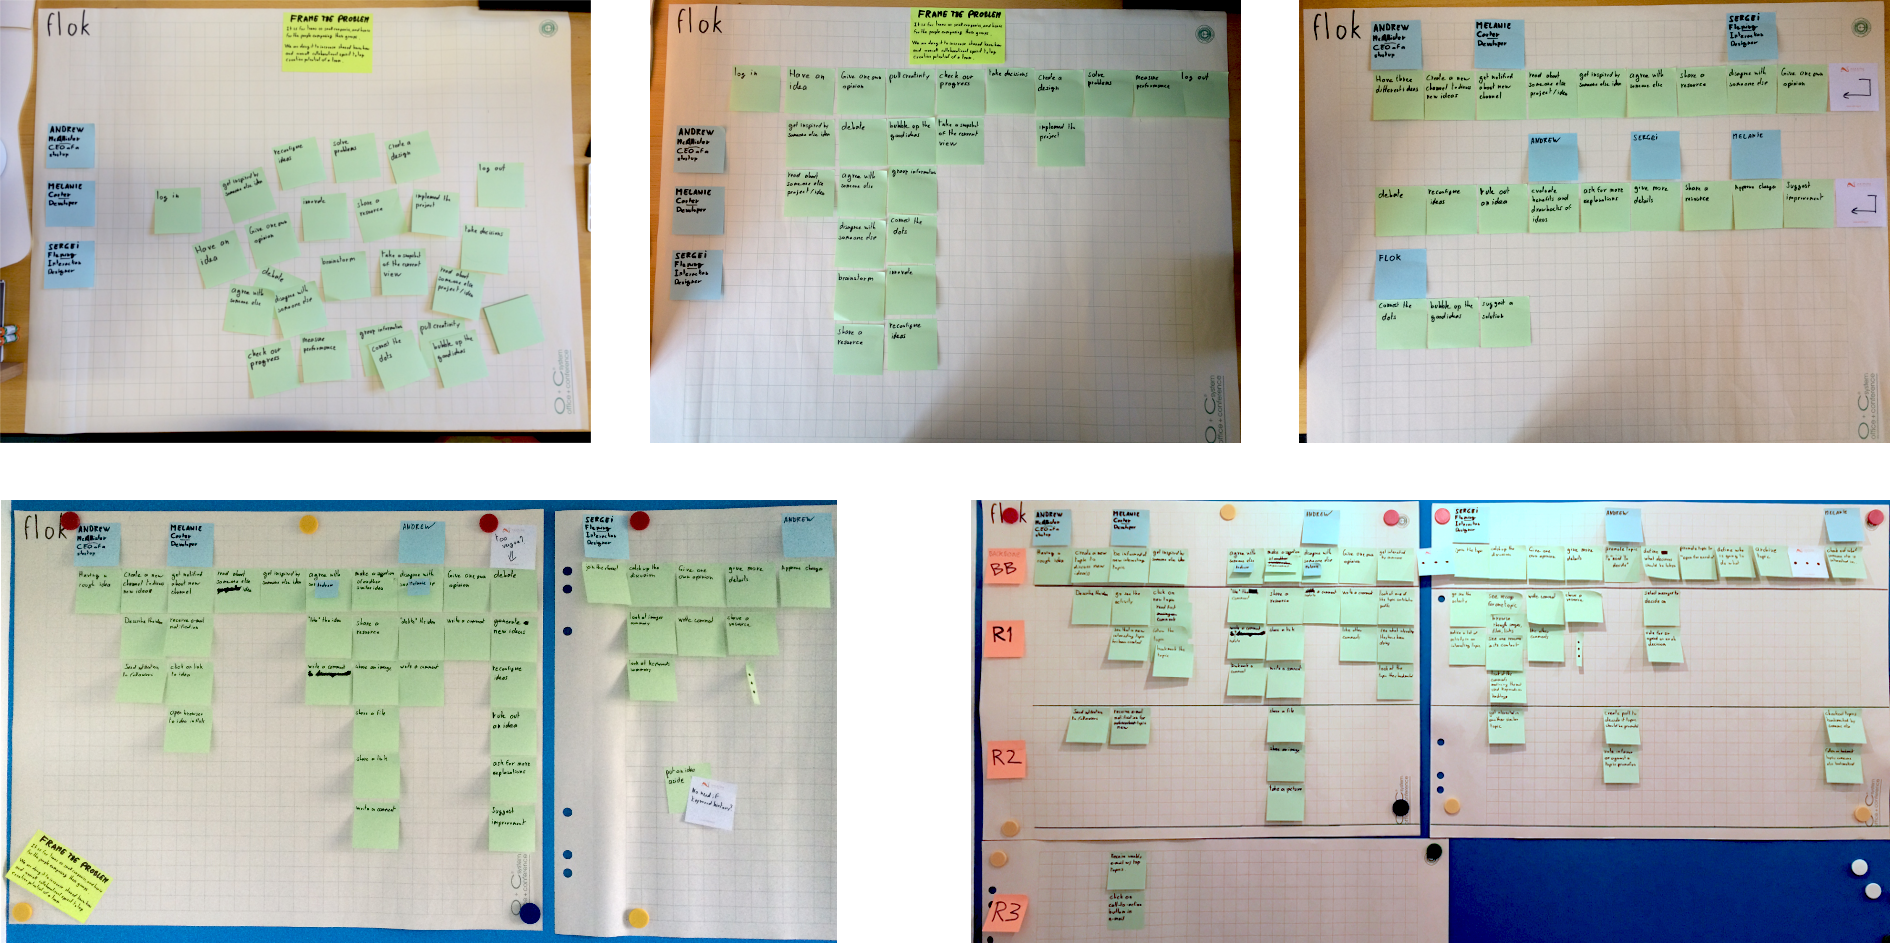
\includegraphics[width=\textwidth]{images/flokUsmEvolution.png}
\caption{Evolution of the user story map for Flok}
\label{fig.flokUsmEvolution}
\end{figure}

%TODO describe a bit the story map structure and the content of the final state

% Not easy to do a User Story Map because of the real-time aspect of the project (realized while doing USM for Tawuala)

\section{Wireframing}

\section{Prototyping}

\section{Front-end implementation}
\subsection{Architecture}

\subsection{Design decisions}

\section{User testing}

\section{Conclusion}

\clearpage
\bibliographystyle{ieeetr}
\bibliography{main}

\end{document}
